\subsection{Supplementary figures and text}

\begin{figure}
    \begin{center}
      \includegraphics{../illustrations/parameter_estimation_scheme.pdf}
    \end{center}
    \caption{}
    \label{fig:parameter_estimation_scheme}
\end{figure}

Text for Figure 7:

Scheme of initial transcription rate constant estimation protocol. \textbf{1:}
Rate constants for the NAC, UAR and promoter escape are randomly sampled from
a uniform distribution (example values are shown). Of these values, the NAC is
used further to obtain backtracking rates at each template position
(\textbf{3}).  This is done by solving equation \eqref{eq:backtrackingcalc},
inserting for each position the associated AP value for the N25 promoter from
Hsu et al.\ \cite{hsu_initial_2006} (\textbf{2}). The distinct backtracking
rate constants at each position are then combined with the NAC, UAR, and
promoter escape rate constants sampled in step \textbf{1} to obtain a complete
kinetic scheme of initial transcription (\textbf{4}). This scheme is then used
to simulate the kinetics of 100 initial transcription events; from these 100
events the distribution of time spent in abortive cycling is calculated and
compared to measured data from Revyakin et al.\ \cite{revyakin_abortive_2006}
(\textbf{5}). From the distance between the measured distribution and the
simulated distribution, a fitness score is produced. This score is associated
to the three randomly selected rate constants in step \textbf{1}, and is a
measure for how well the kinetic scheme with these rate constants (together
with the AP values) agree with the experimental data. By repeating steps
\textbf{1}-\textbf{5} multiple times, distributions are obtained showing which
values of rate constants have the best fitness to experimental data (Figures
\ref{fig:parameter_estimation_proper} and \ref{fig:extrap_and_GreB_minus_fit}) 
